\chapter{Qualitätsmanagement}
	Zur Sicherung der Qualität wurden verschiedene Strategien kombiniert. Zur automatisierten Qualitätskontrolle wurden Unittests eingesetzt. Die Performance und das Verbindungsverhalten durch Firewalls hindurch wurde durch systematische Tests ermittelt. Die Funktion der Benutzeroberfläche wurde durch regelmässige manuelle Tests in Firefox und Chrome überprüft.
	Die Connection und die Videokommunikation wurden durch regelmässige manuelle Tests zu zweit mit zwei Geräten getestet.
	
	\begin{figure}[H]
		\centering
		{\tiny
			\csvautotabular{../qualityManagement/timelog.csv}
		}
		\caption{Die Aktivität ``Qualitätsmanagement"' fasst Testing und Reviewing
		zusammen.}
	\end{figure}

	\section{Automatisierte Tests}
		\begin{description}
			\item[Unittests]		
			\begin{figure}[H]
				\centering
				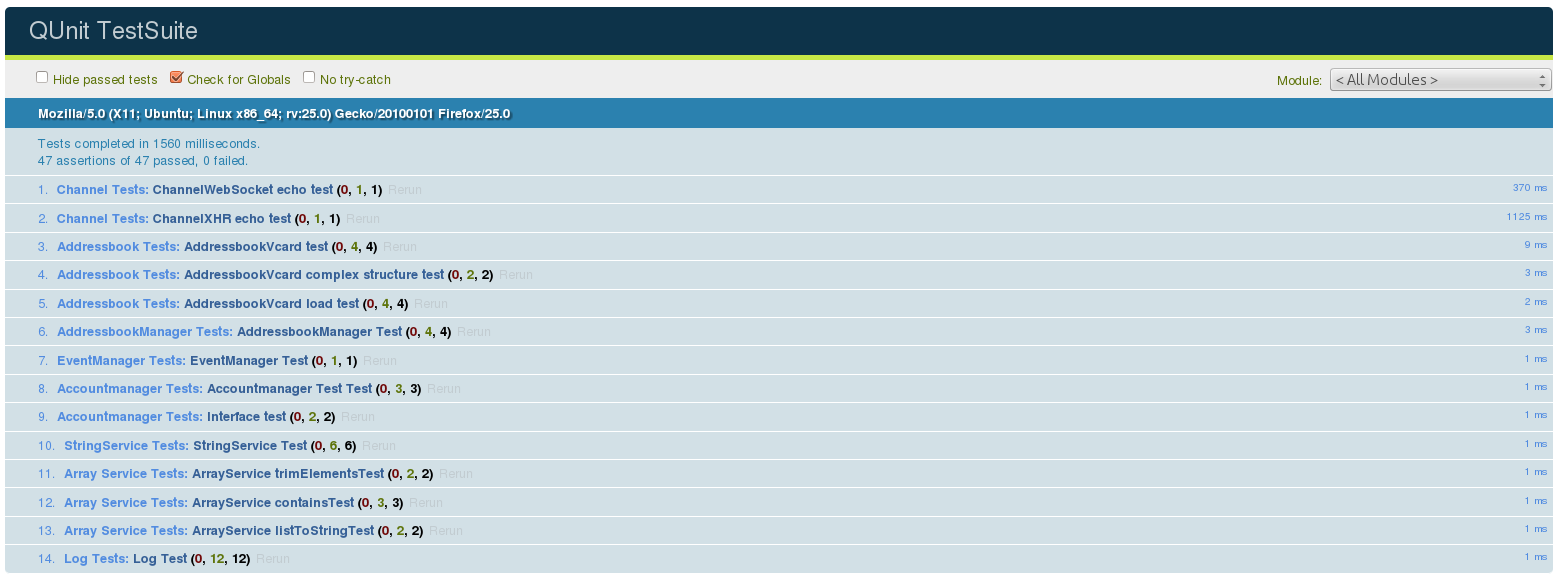
\includegraphics[width=1\textwidth]{../qualityManagement/unittesting.png}
				\caption{mit QUnit erfolgreich ausgeführte Tests}
				\label{unittests}
			\end{figure}
			Die Applikationsdomain wird mit Unittests getestet und die fortbleibende
			Funktion bei Änderungen damit nachgewiesen.
		\end{description}
		
	\section{Systematische Tests}
		\begin{description}
			\item[Performancetest]
			Die Performance wurde durch eine umfangreiche Performanceanalyse untersucht und dokumentiert. Dabei wurden Mobilgeräte wie Desktopgeräte getestet.
		
			Siehe Anhang \ref{performanceanalyse}
		
			\item[Firewall Tests]
			Das Verhalten der durch WebRTC genutzten Protokolle durch Firewalls hindurch wurde in einem dreiteiligen Firewall-Test ermittelt. Dabei wurde das Verhalten der HSR Firewall, von Firewalls in Mobilfunk- und von Firewalls in Heimnetzanbindungen untersucht. 
		
			Siehe Anhang \ref{firewalltests}
		\end{description}
		
	\section{Manuelle Tests}
		\begin{description}
			\item[Connection \& Videoverbindung]
			Die Connection stellt die am schwierigsten zu testende Komponente und gleichfalls eine der komplexeren dar, weil sie die RTCPeerConnection, die RTCDataChannel und die UserMedia Schnittstelle verwendet. Die Schnittstellen interagieren mit dem User und mit Netzwerkevents. Testen mit Unittests wäre nur möglich gewesen, wenn für diese Schnittstellen komplette Dummies gebaut worden wären. 
		
			Aus diesem Grund wurde als Teststrategie manuelles Testen gewählt. Dabei wurden Verbindungsaufbau und -abbau jeweils in jeder Richtung mit Firefox, Chrome und Firefox-Chrome kombiniert sowie allen Variationen von Auf- und Abbaureihenfolgen zu zweit mit zwei Geräten durchgetestet.
	
			Dies wurde in jeder Iteration mindestens einmal durchgeführt um die Funktionalität zu überprüfen.
		
			\item[Kontaktbuch Import] Die Verarbeitung der Kontaktbuchdaten und das Kontaktbuchmanagement haben wir durch Unittests abgedeckt.
			Beim Import hätten wir ebenfalls einen Dummy bauen müssen. Daher wurde auch diese manuel getestet.
		\end{description}
			
		
	\section{Reviews}
		Regelmässige Reviews stellten die Qualität von Dokumentation und Code sicher. Für die Reviews wurde die Commit-Kommentarfunktion von GitHub genutzt.
		
		Zusätzlich hat uns Herr Bläser ein Code Review durchgeführt.
